\begin{figure*}[ht]
\centering
\begin{minipage}{0.9\textwidth}
\centering
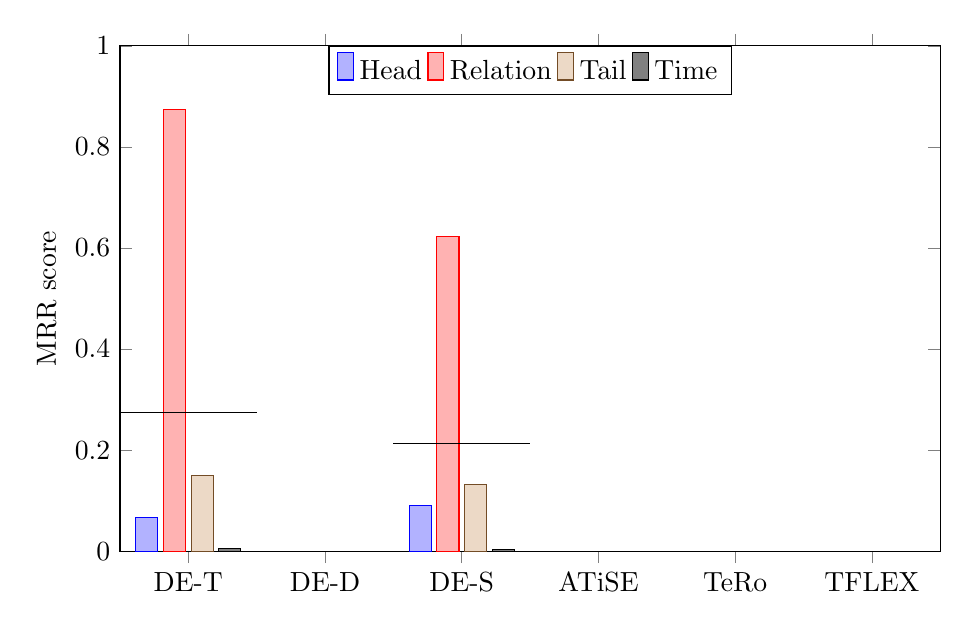
\begin{tikzpicture}
\begin{axis}[
    ybar,
    bar width=8pt,
    xticklabels={x,DE-T,DE-D,DE-S,ATiSE,TeRo,TFLEX},
    ymin=0,
    ymax=1.0,
    ylabel={MRR score},
    height=8cm,
    width=12cm,
    legend style={
        at={(0.5,1.0)},
        anchor=north,
        legend columns=-1
    },
    legend image code/.code={
        \draw [#1] (0cm,-0.1cm) rectangle (0.2cm,0.25cm); },
    ]
\addplot coordinates { %head
(0, 0.06598500048947091) %DE_TransE
(1, 0) %DE_DistMult
(2, 0.0910450302298716) %DE_SimplE
(3, 0) %ATISE
(4, 0) %TERO
(5, 0) %TFLEX
} ;
\addplot coordinates { %relation
(0, 0.8732498916341577) %DE_TransE
(1, 0) %DE_DistMult
(2, 0.6221168235391219) %DE_SimplE
(3, 0) %ATISE
(4, 0) %TERO
(5, 0) %TFLEX
} ;
\addplot coordinates { %tail
(0, 0.15003600005950565) %DE_TransE
(1, 0) %DE_DistMult
(2, 0.13284767704545358) %DE_SimplE
(3, 0) %ATISE
(4, 0) %TERO
(5, 0) %TFLEX
} ;
\addplot coordinates { %time_from
(0, 0.005387766857512553) %DE_TransE
(1, 0) %DE_DistMult
(2, 0.00411020285253353) %DE_SimplE
(3, 0) %ATISE
(4, 0) %TERO
(5, 0) %TFLEX
} ;
\addplot[black,sharp plot,update limits=false,] coordinates { %DE_TransE
(-0.5, 0.27366466476016243)
(0.5, 0.27366466476016243)
} ;
\addplot[black,sharp plot,update limits=false,] coordinates { %DE_DistMult
(0.5, 0)
(1.5, 0)
} ;
\addplot[black,sharp plot,update limits=false,] coordinates { %DE_SimplE
(1.5, 0.21252993341674445)
(2.5, 0.21252993341674445)
} ;
\addplot[black,sharp plot,update limits=false,] coordinates { %ATISE
(2.5, 0)
(3.5, 0)
} ;
\addplot[black,sharp plot,update limits=false,] coordinates { %TERO
(3.5, 0)
(4.5, 0)
} ;
\addplot[black,sharp plot,update limits=false,] coordinates { %TFLEX
(4.5, 0)
(5.5, 0)
} ;
\legend{Head,Relation,Tail,Time}
\end{axis}
\end{tikzpicture}
\caption{yago11k, split 3}
\label{fig:compare_yago11k_3}
\end{minipage}
\end{figure*}
